\begin{center}
  \Large
  \textbf{BIOGRAFI PENULIS}
\end{center}

\addcontentsline{toc}{chapter}{BIOGRAFI PENULIS}

\vspace{2ex}

\begin{wrapfigure}{L}{0.3\textwidth}
  \centering
  \vspace{-3ex}
  % Ubah file gambar berikut dengan file foto dari mahasiswa
  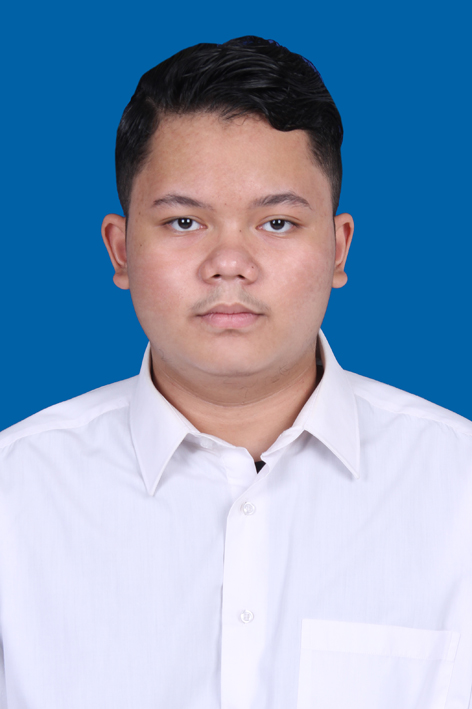
\includegraphics[width=0.3\textwidth]{gambar/evan.jpg}
  \vspace{-4ex}
\end{wrapfigure}

% Ubah kalimat berikut dengan biografi dari mahasiswa
\name{}, lahir di Bandung pada tanggal 24 September 2002. Penulis merupakan anak pertama dari lima bersaudara yang tinggal dan besar di Depok, Jawa Barat. Setelah lulus dari SMA Negeri 8 Depok, penulis kemudian melanjutkan pendidikan ke jenjang Strata Satu (S1) di Departemen Teknik Komputer, Fakultas Teknologi Elektro dan Informatika Cerdas, Institut Teknologi Sepuluh Nopember mulai dari tahun 2020. 

Penulis merupakan orang yang aktif berorganisasi dan memiliki berbagai \emph{softskill} serta \emph{hardskill}. Hal ini dibuktikan dari rekam jejak organisasi dan keprofesian dari penulis seperti Staff Humas \emph{Multimedia and Game Event} (MAGE) 8 ITS, Staff Riset dan Keprofesian Himpunan Mahasiswa Teknik Komputer ITS (HIMATEKKOM ITS), Asisten Lab \emph{Multimedia Internet of Things} Teknik Komputer ITS (M-IOT), dan \emph{Embedded Firmware Developer Intern} di PT Len Industri (Persero).